%______________________________________________________________________________
% main.tex

\input{preamble12-screen.tex}
\hypersetup{%
    pdfauthor={Mike Pierce}%
   ,pdftitle={Math N16B Homework Seven, Summer 2021}%
   ,pdfkeywords={Pierce,MathN16B,16B,N16B,Calculus,Integration,Berkeley}%
}
\usepackage{fourier}
\input{accessible-colors.tex}
\input{newcommand.tex}
\input{newenvironment.tex}
\pagestyle{empty}


\begin{document}

\begin{center}
    {\Huge{Homework Seven}}
    \\ \footnotesize{Analytic Geometry and Calculus}
    \\ \footnotesize{UC Berkeley Math N16B, Summer 2021}
\end{center}
\vspace{2em}

Upload your responses to the prompts marked
(\textsc{\textcolor{magenta}{Submit}})
to Gradescope before 8pm Friday; 
you will receive feedback on these.
\begin{center}
    \href{https://www.gradescope.com/courses/275664}%
    {\texttt{gradescope.com/courses/275664}}
\end{center}
The rest of the exercises you should complete at your discretion.
Note that \emph{Calculus with Applications, 11th Edition} 
has some select solutions, usually to odd-numbered exercises, in the back.


\section*{Goals this Week}

Here are some goals you should have in mind while exercising:
\begin{enumerate}
    \item 
        You've gotta know what if means for a function to be a 
        \term{probability density function} (PDF) 
        and how a \term{cumulative distribution function} (CDF)
        relates to its corresponding PDF via the Fundamental Theorem of Calculus. 

    \item 
        You should gain some heavy familiarity with the basic vocabulary
        of calculus-based probability.
        Know what the \term{expected value} (\term{mean}), \term{median},
        \term{variance}, and \term{standard deviation} 
        of a continuous random variable are,
        and how to calculate these from the PDF of that random variable.
        Know what a \term{uniform}, \term{exponential}, 
        and \term{normal} distribution are, 
        and what the \term{$z$-score} of a value of a normally distributed
        random variable is.

\end{enumerate}

\newpage

\section*{Exercises}

\begin{enumerate}
    \item % 11.1 Continuous Probability
        Remember a PDF is a continuous function $f$ defined on some domain $[a,b]$
        (where $a$ and $b$ might be infinite) 
        such that (1) $f(x)$ is positive for all $x$ between $a$ and $b$,
        and (2) $\int_a^b f(x) \dx =1 $. 
        The initial exercises from Chapter 11.1 of
        \emph{Calculus with Applications, 11th Edition}
        only serve to reinforce this definition by
        making you do some contrived exercises. 
        Do those exercises if it helps, 
        but the important thing is to understand
        \emph{why} a PDF is defined the way it is.
        Also, understand that if a function is positive on some interval
        you can always \emph{make it} a PDF by rescaling it.

    \item % 11.2 Expected Value and Variance
        The initial exercises from Chapter 11.2 of 
        \emph{Calculus with Applications, 11th Edition}
        provides some good practice at calculating 
        expected value, variance, standard deviation, etc. 
        Do as many as you need to feel confident with these calculations.

    \item 
        (\textsc{\textcolor{magenta}{Submit}})
        The definition of the variance of a random variable $X$
        with PDF $f$ and domain $[a,b]$ is given by
        \begin{equation*}
            \int\limits_a^b (x-\mu)^2 f(x) \dx
        \end{equation*}
        where $\mu$ is the expected value (mean) of $X$.
        But there's an easier formula for the variance. 
        Prove that
        \begin{equation*}
            \int\limits_a^b (x-\mu)^2 f(x) \dx
            \;\;=\;\;
            \int\limits_a^b x^2 f(x)\dx - \mu^2
            \,.
        \end{equation*}
        \textsc{Hint}: remember the \emph{definition} of $\mu$.
        
    %\item 
    %    For some point $p$ chosen at random in the half-disk of radius $2$,
    %    let $X$ denote it's distance to the origin.
    %    What is the probability density function for $X$?
    %    %TODO
    %    \begin{center}
    %        \includegraphics[width=0.96\textwidth]{screenshots/half-disk.png}
    %    \end{center}

    \item % 11.3 Special PDFs: Uniform, Normal, z-Scores
        Again, the initial exercises from Chapter 11.3 of 
        \emph{Calculus with Applications, 11th Edition}
        are silly, but do serve to reinforce the definitions from this section.
        Do as many of these exercises as you need to
        know what the uniform, exponential, and normal distributions are,
        and what a $z$-score is.

    \item 
        These exercises from the textbook are all basically the same exercise
        over and over, but are still meaningful and demonstrate the purpose 
        of calculus-based probability.
        \begin{center}
            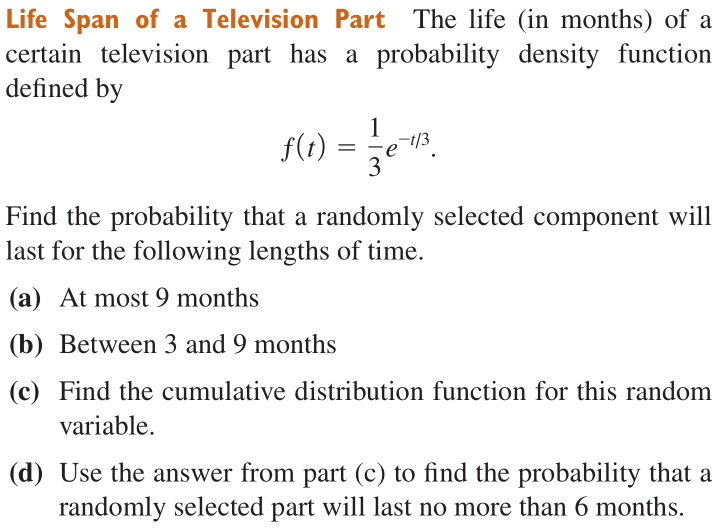
\includegraphics[width=0.96\textwidth]{screenshots/television.png}
        \end{center}
        \newpage
        (\textsc{\textcolor{magenta}{Submit}})
        everything about these blood clots:
        \begin{center}
            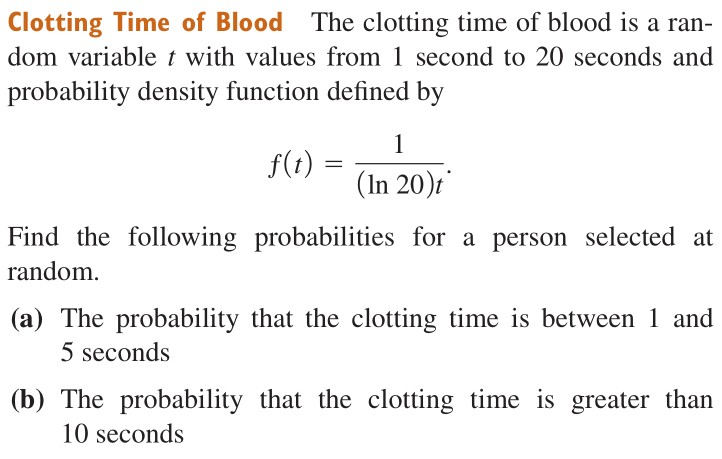
\includegraphics[width=0.96\textwidth]{screenshots/blood1.png}
            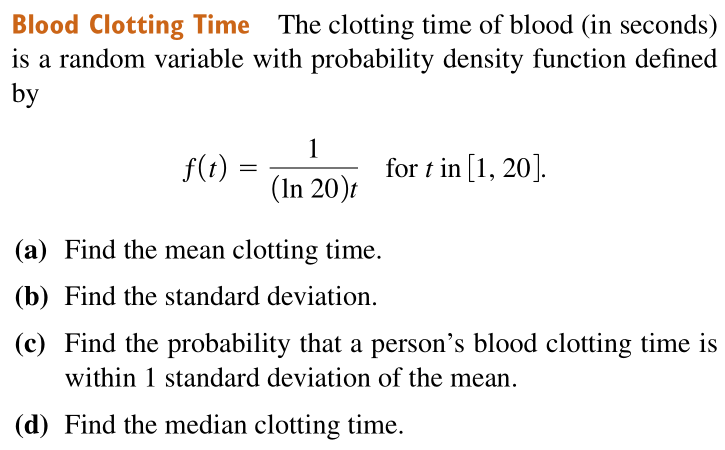
\includegraphics[width=0.96\textwidth]{screenshots/blood2.png}
        \end{center}
        \newpage
        \begin{center}
            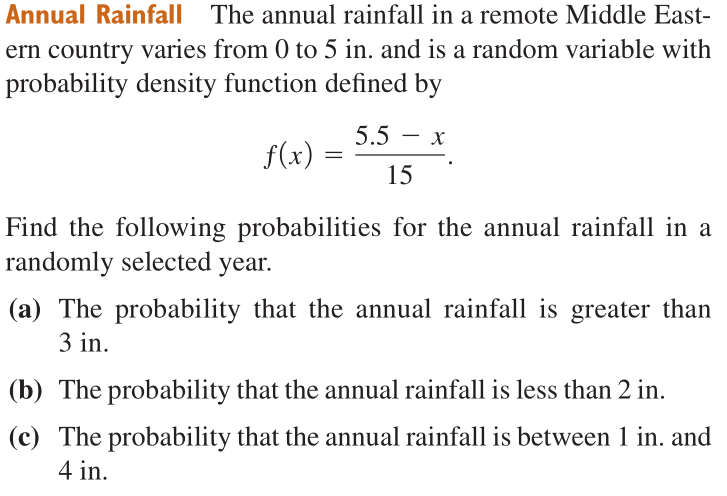
\includegraphics[width=0.96\textwidth]{screenshots/rainfall1.png}
            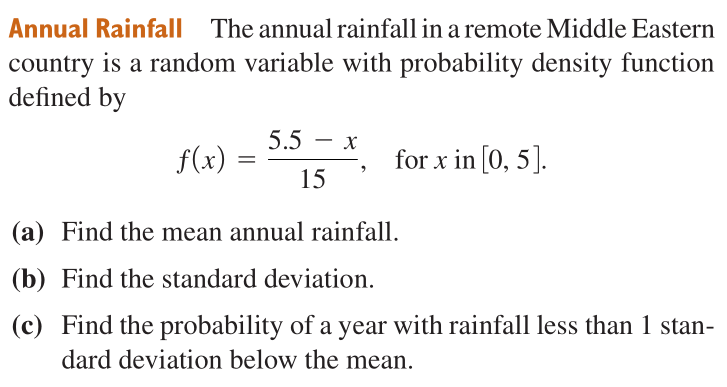
\includegraphics[width=0.96\textwidth]{screenshots/rainfall2.png}
            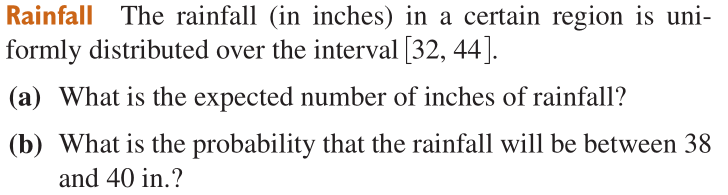
\includegraphics[width=0.96\textwidth]{screenshots/rainfall3.png}
        \end{center}
        \newpage
        (\textsc{\textcolor{magenta}{Submit}})
        everything about these earthquakes:
        \begin{center}
            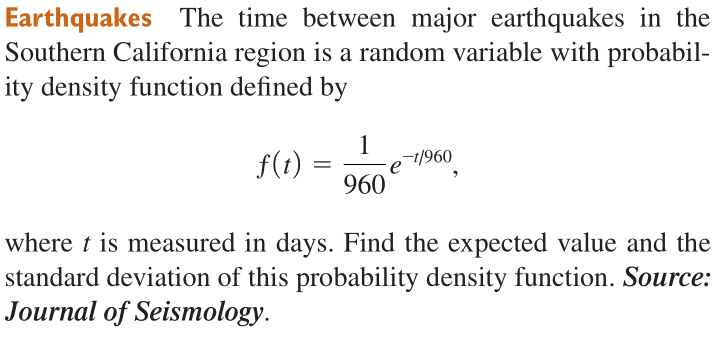
\includegraphics[width=0.96\textwidth]{screenshots/earthquakes1.png}
            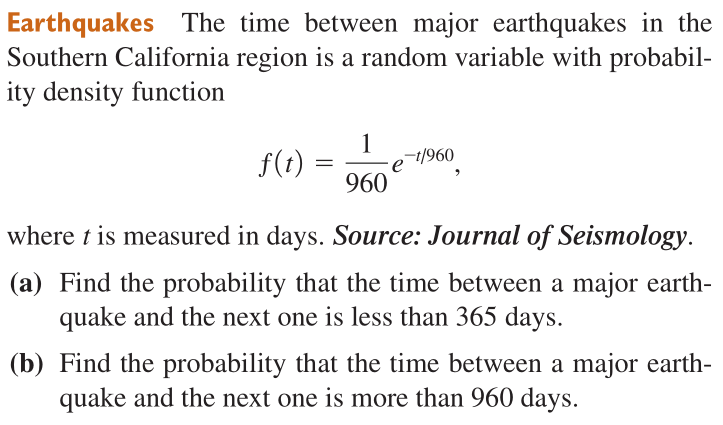
\includegraphics[width=0.96\textwidth]{screenshots/earthquakes2.png}
        \end{center}
        \newpage
        \begin{center}
            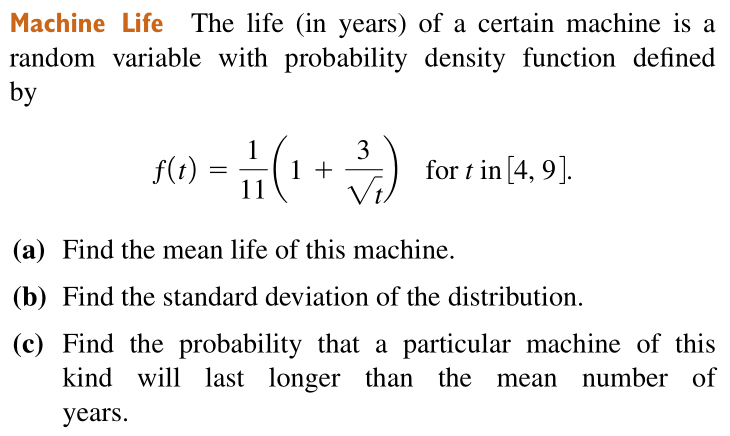
\includegraphics[width=0.96\textwidth]{screenshots/machine.png}
            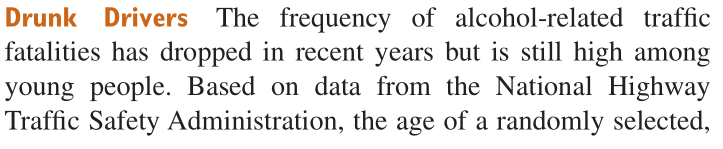
\includegraphics[width=0.96\textwidth]{screenshots/drunk1.png}
            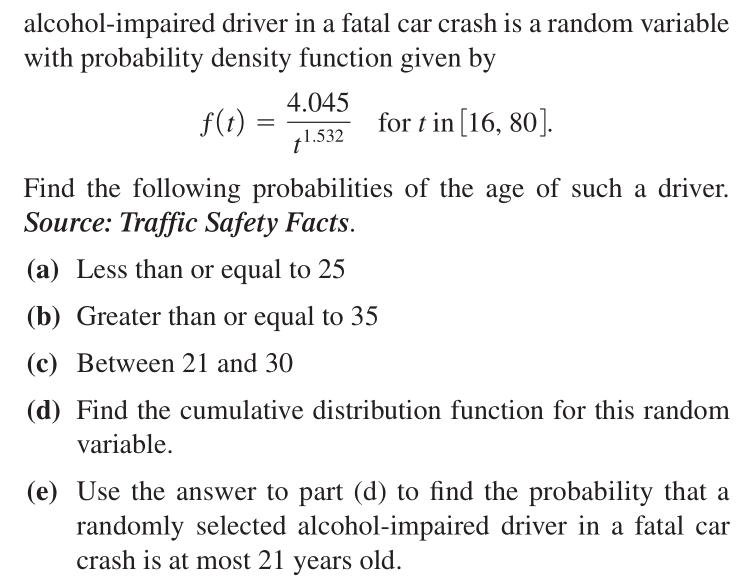
\includegraphics[width=0.96\textwidth]{screenshots/drunk2.png}
            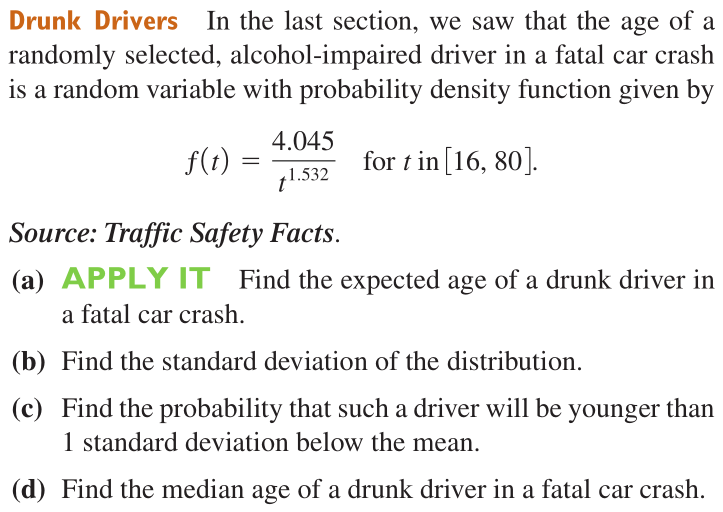
\includegraphics[width=0.96\textwidth]{screenshots/drunk3.png}
        \end{center}

    \item 
        (\textsc{Recreation})
        There's a map of the world 
        that has every single town in the world marked on it. 
        For each town on this map you draw a straight line connecting it to its nearest neighboring town 
        (nearest in terms of distance along a straight line, \emph{not} distance along roads).
        Show that after you've done this for every town on the map, 
        each town can be connected to at most five others.

\end{enumerate}

\end{document}

